\section{Reviewer 1}

\subsection{Major Comments}

\begin{enumerate}
	\item  The dataset suffers from two notable issues with regard to a fair comparison between ERGM, LSM, and the proposed AME approach ... To address both issues, the authors could either describe in detail the merits and demerits of this empirical application for comparing AME to existing frameworks, or could draw up a simple simulation to show the sensitivity of the model comparison results to the factors identified above.
	\begin{itemize}
		\item The first is that each node’s latent position is likely to be correlated with the model terms of interest – a point raised by Cranmer et al. as well (pp. 248-9). In this case, key government players have lower Euclidean distances because they tend to be positioned in the center of the latent space. If this were not the case, would we see such a large divergence between the LSM and AME results? For example, would the AME perform much ``better'' than the LSM if the network data exhibited a less hierarchial/more egalitarian structure? 
			\begin{itemize}
				\item \textcolor{blue}{ \emph{
				To answer this question we conduct a simulation exercise -- included in the appendix. Specifically, we set up six simulation scenarios representing varying degrees of ``egalitarianism'' in terms of network structure. For each scenario, we simulate 50 networks with 100 nodes each and then evaluate the performance of AME (specifically, the LFM portion) and LSM to predict this network structure. The results are shown in Figure 8 of the appendix and included below in Figure~\ref{fig:sim_egal} as well. Each panel here represents one scenario in which we vary the extent to which the degree distribution is egalitarian. The left most panel represents the situation in which the structure of the network is most egalitarian. Next, we run an AME (specifically, the LFM portion) and LSM on each of the simulated networks from each scenario and compare the predictive performance based on AUC (ROC) and AUC (PR).\footnote{The additive effects from the SRM were excluded for AME to make the test more fair.} We set $K=2$ for both the AME and LSM. The results of this analysis indicate that under each scenario AME performs better than LSM. However, the performance of both models tends to decline as the structure of the simulated networks become less egalitarian (i.e., the extent of tie formation among just a few nodes becomes much higher than the typical node in the network).  
				}}
			\end{itemize}	
			\begin{figure}[ht]
				\centering
				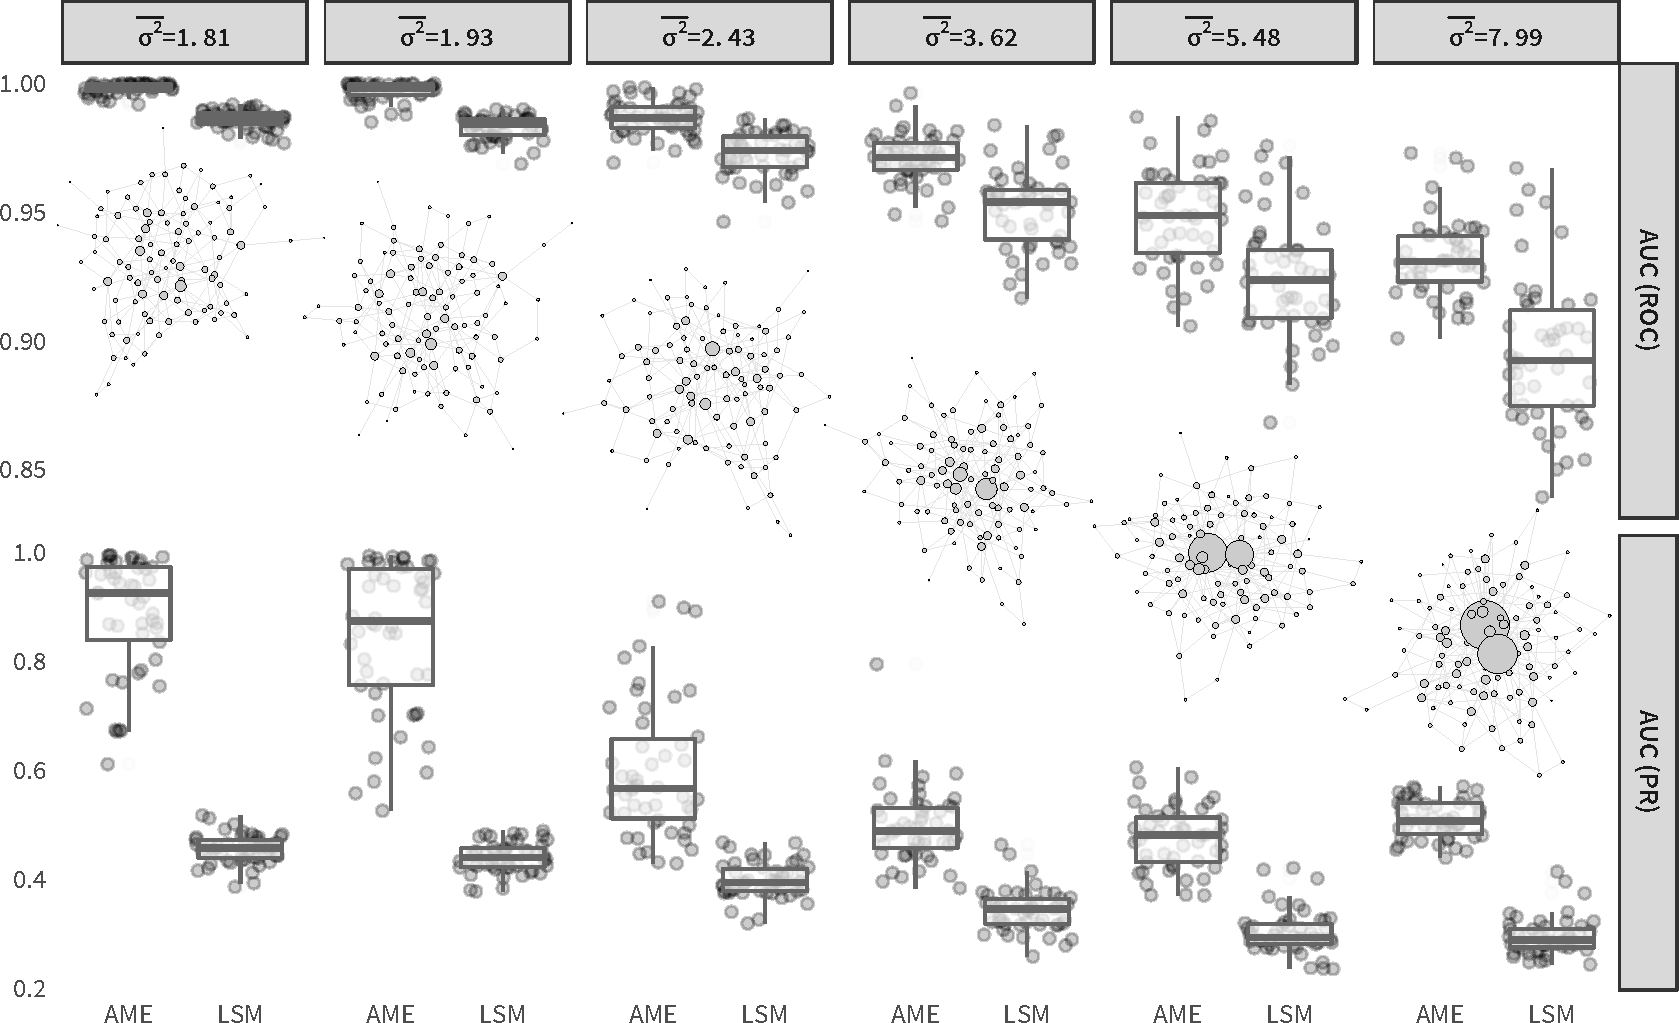
\includegraphics[width=1\textwidth]{sim1Viz_nets.pdf}
				\caption{Predictive performance of AME vs LSM for networks under five scenarios (the panels) that vary the extent to which the distribution of ties are egalitarian. We use a box plot to represent the performance of AME and LSM across fifty simulations for each scenario. The set of network visualizations across the diagonal of the plot illustrate a representative network from one simulation under that scenario, and the size of nodes corresponds to their number of ties. The labels at the top of each panel indicate the standard deviation of the number of ties, which are averaged across the fifty simulations for that scenario.}
				\label{fig:sim_egal}	
			\end{figure}			
		\item The second is that the data exhibit high reciprocity such that the directed network is effectively a symmetric undirected network. How would the results differ for a more evenly-balanced directed network (i.e. one where the probability of a reciprocal tie is 50\%)? 
			\begin{itemize}
				\item \textcolor{blue}{ \emph{
				To answer this question we again conduct a simulation exercise -- included in the appendix. Here the simulation scenarios vary the level of reciprocity. For each scenario, we again simulate 50 binary, directed networks. The results are included in Figure 9 of the append and shown in Figure~\ref{fig:sim_recip}. Each panel here represents represents one scenario with a certain degree of reciprocity. The left-most panel highlights the case where there is little to no reciprocity in the network and the right-most where the level of reciprocity is quite high. The average level of reciprocity across the fifty simulated networks is given at the top of each panel. To compare AME and LSM, we again utilize AUC (ROC) and AUC (PR) statistics. $K=2$ for both models and no covariate information is provided.\footnote{The AME is run without the additive effects portion from the SRM to make the test more fair.} Here again we find that the AME consistently outpeforms the LSM, though at higher levels of reciprocity the performance difference between the two approaches does shorten. 
				}}
			\end{itemize}	
			\begin{figure}[ht]
				\centering
				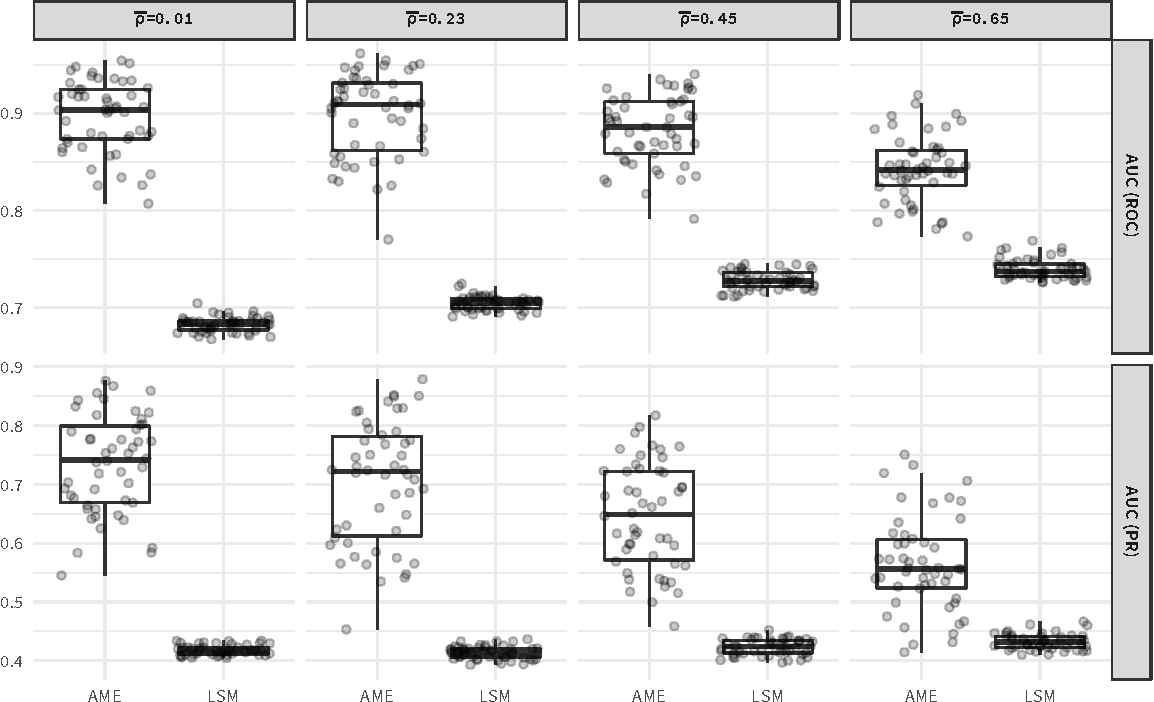
\includegraphics[width=1\textwidth]{sim2Viz.pdf}
				\caption{Predictive performance of AME vs LSM for networks with varying levels of reciprocity. We use a box plot to represent the performance of AME and LSM across fifty simulations for each scenario. The labels at the top of each panel indicate the average level of reciprocity across the fifty simulated in that scenario.}
				\label{fig:sim_recip}		
			\end{figure}
	\end{itemize}
\end{enumerate}

\subsection{Minor Comments}

\begin{enumerate}
	\item It would be helpful for the reader to compare AME to non-network models as well, so the authors could include a column in Table 3 for results from a logit model (or the like). 
	\begin{itemize}
		\item \textcolor{blue}{ \emph{
		We thank the reviewer for his comments and have included a logit model for comparison. Figure 2 in the paper shows that the Logit model performs notable worse in terms of out-of-sample predictive performance than the AME.
		}}
	\end{itemize}		
	\item Typo on page 13, first sentence should read: $y = B'x - |u_i – u_j|$ instead of $y = B'x + |u_i - u_j|$.
	\begin{itemize}
		\item \textcolor{blue}{ \emph{
		We thank the reviewer for his comments and have fixed this typo.
		}}
	\end{itemize}		
\end{enumerate}

